%Refferences used in this section:
%\cite{STMicroelectronics}
%\cite{PCorporation}
%\cite{DCook}
%\cite{DMcRoberts}
%\emph{edited from image by Biezl}\cite{Biezl}
%\cite{PAndersen}

\section{H-Bridge}\label{sec:HBridge}
The H-bridge see \figref{Hbridge} is a circuit used for motor control. To control the motor some FETs are controlled with a PWM signal. The duty cycle of this PWM signal determines at which velocity the motor will run.\cite{DCook}

\begin{figure}[H]
	\centering
	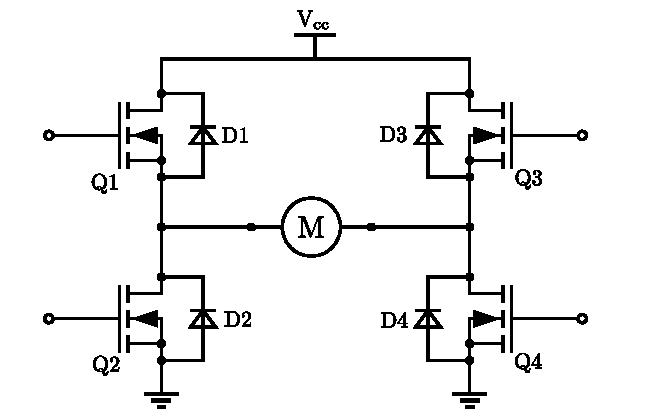
\includegraphics[scale=.6]{figures/Hbridge.pdf}
	\caption{Standard H-bridge.\\ \emph{Edited from image by Biezl}.\cite{Biezl}}
	\label{Hbridge}
\end{figure}\vspace{-5mm}

There exists a wide range of configurations in which the H-bridge can be implemented. These configurations determines the modes of operation, where each mode has some different properties. Some of the common modes are described in the following sections.\cite{DCook}

\subsection{Regenerative Coast Mode}
One mode of operation is the coast mode, where the PWM signal controls 2 of the 4 FETs, Q1 and Q3, as seen on \figref{HbridgeClockwiseCoastON}. In the on-period of the PWM signal the Q1 and Q4 are turned on, leading the current from Vcc through the motor and down to ground. This means that the motor is driven by the supply when the PWM goes high. When the PWM goes low, both Q1 and Q4 are shut off. Given that Q2 and Q3 are permanently off, the current generated by the motor in its armature coils will be driven through the intrinsic diodes of Q2 and Q3. So when the PWM goes low, the battery is charged.\cite{PAndersen}

  \begin{minipage}{\linewidth}
  	\begin{minipage}{0.45\linewidth}
  		\begin{figure}[H]
  			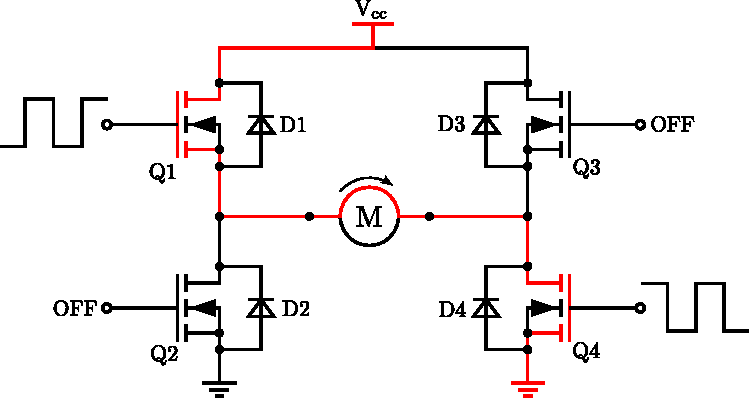
\includegraphics[scale=.6]{figures/HbridgeClockwiseCoastON.pdf}
  			\centering
  			\vspace{-.4cm}
  			\captionsetup{justification=centering}
  			\captionof{figure}{Clockwise coast in on-state.\\ \emph{Edited from image by Biezl}.\cite{Biezl}}
  			\label{HbridgeClockwiseCoastON}
  		\end{figure}\vspace{-5mm}
  	\end{minipage}
  	\hspace{0.03\linewidth}
  	\begin{minipage}{0.45\linewidth}
  		\begin{figure}[H]
  			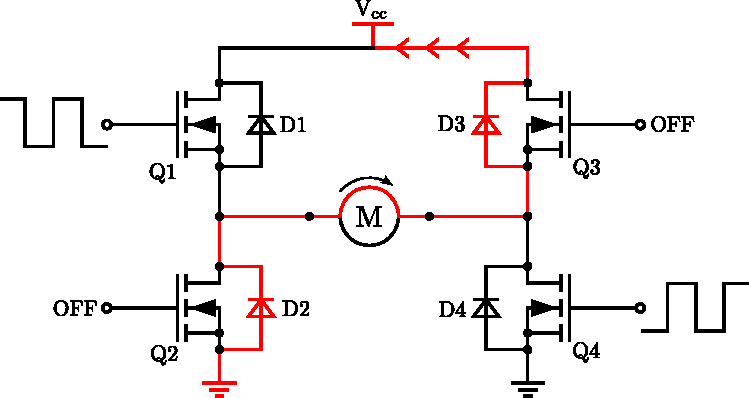
\includegraphics[scale=.6]{figures/HbridgeClockwiseCoastRegen.pdf}
  			\centering
  			\vspace{-.4cm}
  			\captionsetup{justification=centering}
  			\captionof{figure}{Clockwise coast in off-state.\\ \emph{Edited from image by Biezl}.\cite{Biezl}}
  			\label{HbridgeClokwiseCoastRegen}
  		\end{figure}\vspace{-5mm}
  	\end{minipage}
  \end{minipage}

\subsection{4Q Mode}
In this mode of operation the PWM signal is imposed on all 4 FETs, as seen on \figref{HbridgeClokwise4Q} and \figref{HbridgeCounterClokwise4Q}. On \figref{HbridgeClokwise4Q}, Q1 and Q4 are turned on by the PWM signal, allowing current to pass through the motor from Vcc to ground. Although the same PWM signal is imposed on the 4 FETs, only two can be turned on at the time, due to the NOT-gate placed on the gate of Q2 and Q3. Comparing \figref{HbridgeClokwise4Q} and \figref{HbridgeCounterClokwise4Q}, it is seen that the polarity across the motor is switched between the up- and down-period of the PWM.\cite{PAndersen}

  \begin{minipage}{\linewidth}
  	\begin{minipage}{0.45\linewidth}
  		\begin{figure}[H]
  			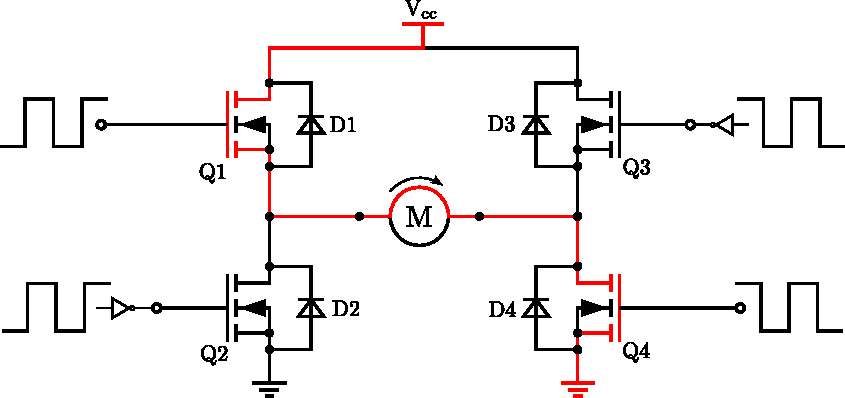
\includegraphics[scale=.53]{figures/HbridgeClockwise4Q.pdf}
  			\centering
  			\vspace{-.4cm}
  			\captionsetup{justification=centering}
  			\captionof{figure}{Clockwise 4Q operation.\\ \emph{Edited from image by Biezl}.\cite{Biezl}}
  			\label{HbridgeClokwise4Q}
  		\end{figure}\vspace{-5mm}
  	\end{minipage}
  	\hspace{0.03\linewidth}
  	\begin{minipage}{0.45\linewidth}
  		\begin{figure}[H]
  			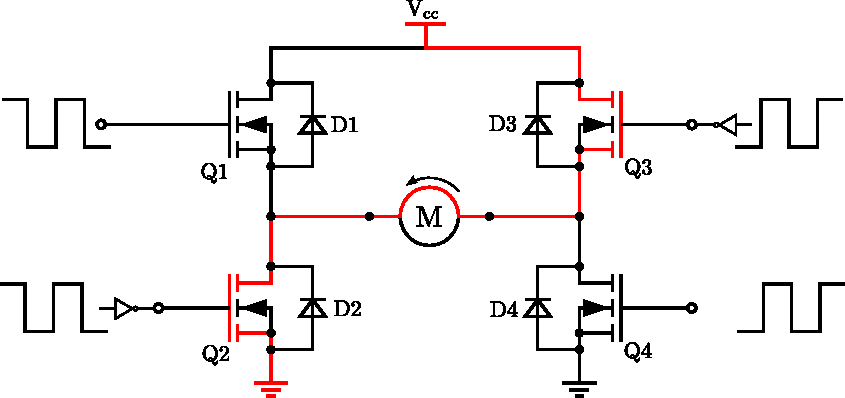
\includegraphics[scale=.53]{figures/HbridgeCounterClockwise4Q.pdf}
  			\centering
  			\vspace{-.4cm}
  			\captionsetup{justification=centering}
  			\captionof{figure}{Counterclockwise 4Q operation.\\ \emph{Edited from image by Biezl}.\cite{Biezl}}
  			\label{HbridgeCounterClokwise4Q}
  		\end{figure}\vspace{-5mm}
  	\end{minipage}
  \end{minipage}

With this mode of operation a duty cycle of \si{50 \%} makes the motor stand still, less than \si{50 \%} will make it turn one way and more than \si{50 \%}, the other way.

\subsection{Brake Mode}
This mode of operation imposes the PWM signal on one side of the H-bridge, as seen on \figref{HbridgeClockwiseBrakeON} and \figref{HbridgeClockwiseBrakeOFF}. The PWM signal in collaboration with the NOT-gate shifts between Q1 and Q2, which provides the two current paths as shown. On \figref{HbridgeClockwiseBrakeON} the motor is driven by the supply, connected through Q1 and Q4. On \figref{HbridgeClockwiseBrakeOFF} the motor is short-circuited to ground through Q2 and Q4, which brakes on the motor. In this example the configuration brakes to ground, however the principal is the same when braking to to Vcc.\cite{PAndersen}

  \begin{minipage}{\linewidth}
  	\begin{minipage}{0.45\linewidth}
  		\begin{figure}[H]
  			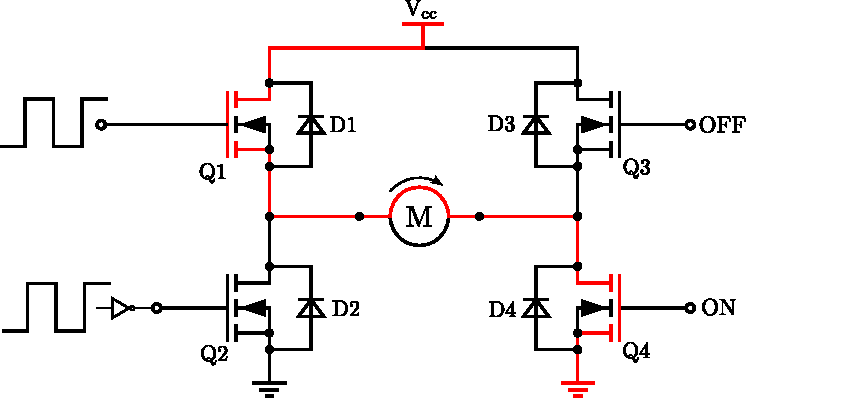
\includegraphics[scale=.6]{figures/HbridgeClockwiseBrakeON.pdf}
  			\centering
  			\vspace{-.4cm}
  			\captionsetup{justification=centering}
  			\captionof{figure}{Clockwise brake in on-state.\\ \emph{Edited from image by Biezl}.\cite{Biezl}}
  			\label{HbridgeClockwiseBrakeON}
  		\end{figure}\vspace{-5mm}
  	\end{minipage}
  	\hspace{0.03\linewidth}
  	\begin{minipage}{0.45\linewidth}
  		\begin{figure}[H]
  			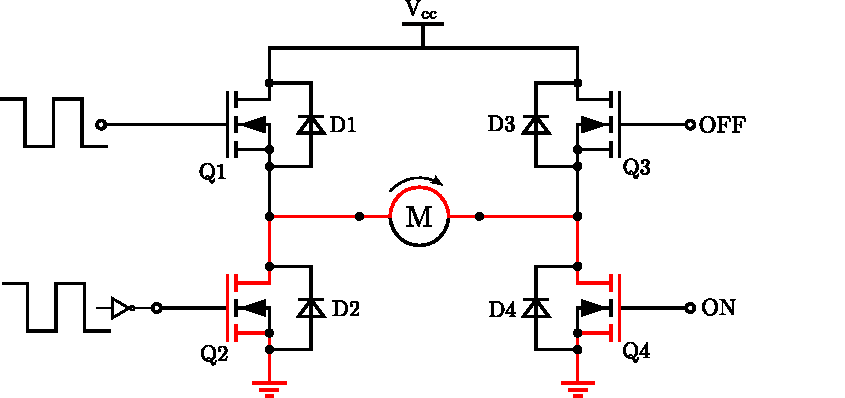
\includegraphics[scale=.6]{figures/HbridgeClockwiseBrakeOFF.pdf}
  			\centering
  			\vspace{-.4cm}
  			\captionsetup{justification=centering}
  			\captionof{figure}{Clockwise brake in off-state.\\ \emph{Edited from image by Biezl}.\cite{Biezl}}
  			\label{HbridgeClockwiseBrakeOFF}
  		\end{figure}\vspace{-5mm}
  	\end{minipage}
  \end{minipage}

There multiple ways to configure an electrical break operation of an H-bridge, in this example the PWM signal is imposed on Q2, rather than only using the intrinsic diode, D2, when in OFF-state, \figref{HbridgeClockwiseBrakeOFF} \cite{DCook}. This method creates less heat dissipation in the FET, however weather it is necessary depends largely on the specifications of the FETs and the current draw of the load.

\subsection{Double H-bridge Brake Mode}
Implemented on the vehicle is a double H-bridge, which is configured to run in brake mode as illustrated on \figref{DoubleHbridgeBrakeON} and \figref{DoubleHbridgeBrakeOFF}. 

\begin{figure}[H]
	\centering
	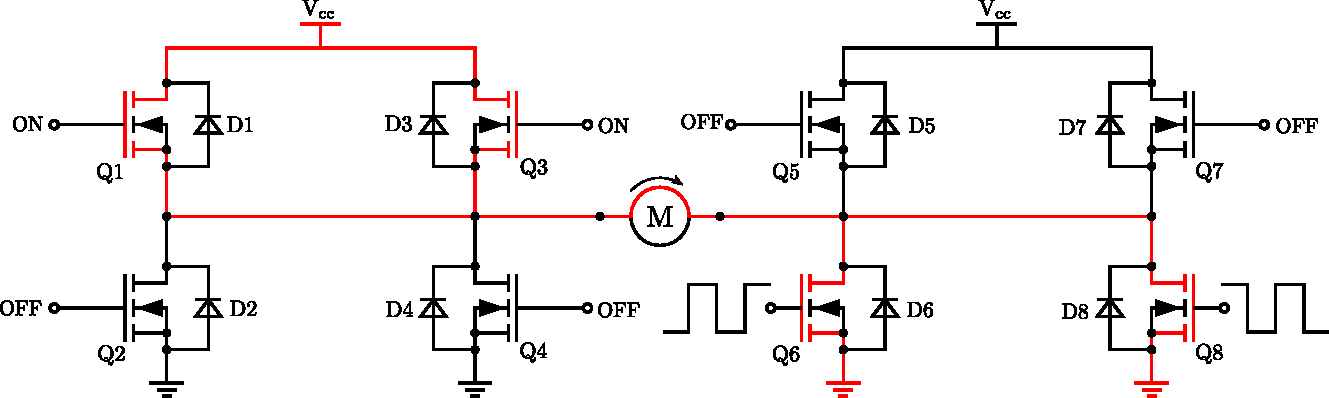
\includegraphics[scale=.6]{figures/DoubleHbridgeBrakeON.pdf}
	\caption{Double H-bridge brake operation in on-state.\\ \emph{Edited from image by Biezl}.\cite{Biezl}}
	\label{DoubleHbridgeBrakeON}
\end{figure}\vspace{-5mm}

In this configuration the PWM signal is only imposed on Q6 and Q8. So instead of activating Q5 and Q7 in the OFF-period, as in \figref{HbridgeClockwiseBrakeOFF}, it utilizes the intrinsic diodes of Q5 and Q7, as shown on \figurename{DoubleHbridgeBrakeOFF}. This can sometimes cause too high heat dissipation in the intrinsic diodes, however this H-bridge has an absolute maximum rating of \si{\pm 30 \ A}, and in this configuration has two FETs in parallel, which is more than sufficient\cite{STMicroelectronics}.

\begin{figure}[H]
	\centering
	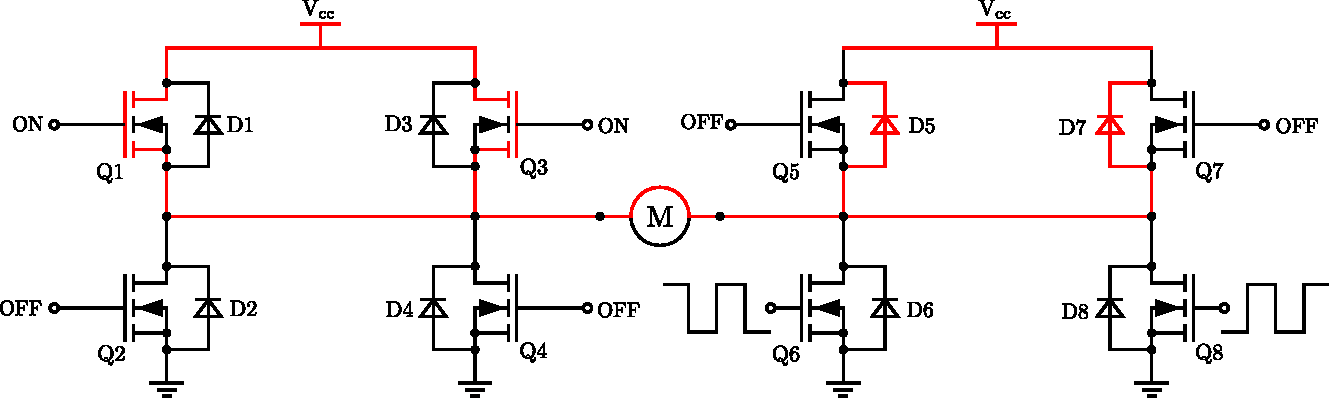
\includegraphics[scale=.6]{figures/DoubleHbridgeBrakeOFF.pdf}
	\caption{Double H-bridge brake operation in off-state.\\ \emph{Edited from image by Biezl}.\cite{Biezl}}
	\label{DoubleHbridgeBrakeOFF}
\end{figure}\vspace{-5mm}

In brake operation the motor breaks in the OFF-period, as opposed to coast operation, where the motor runs freely in the OFF-period of the PWM signal. Though the coast mode is more energy efficient, it is harder to control the vehicle when trying to compensate for too high speeds. An H-bridge in coast operation can add more inertia to the system, however it is not very efficient when the system gains too much inertia, e.g. when going downhill. Break operation on the other hand is less energy efficient, as it dissipates to break in the OFF-period of the PWM. This however allows the H-bridge to both increase and decrease speed, which allows for better control when for instance the vehicle is going downhill.